\documentclass{article}

\usepackage[final]{neurips_2019}

\usepackage[utf8]{inputenc}
\usepackage[T1]{fontenc}
\usepackage{hyperref}
\usepackage{url}
\usepackage{booktabs}
\usepackage{amsfonts}
\usepackage{nicefrac}
\usepackage{microtype}
\usepackage{graphicx}
\usepackage{xcolor}
\usepackage{lipsum}

\newcommand{\note}[1]{\textcolor{blue}{{#1}}}

\title{
  GAN Enabled Drone Trajectory Prediction \\
  \vspace{1em}
  \small{\normalfont Stanford CS236G Final Project} 
}

\author{
  Akram Sbaih \\
  Department of Computer Science \\
  Stanford University \\
  \texttt{akram@stanford.edu} \\
     \And
   \texttt{Mentor} Eric Zelikman \\
   Department of Computer Science \\
   Stanford University \\
   \texttt{ezelikman@cs.stanford.edu} \\
}

\begin{document}

\maketitle

 \begin{abstract}
 Forecasting the possible trajecotries of other drones is important for a drone in a drone-race in order to avoid collision with them. In the other hand, there isn't only one possible trajectory for a drone given its history locations since it has the power to change its own direction. Therefore, I explore in this project training a Transformer GAN that generates a variaty of possible trajectories for the next second of a drone given its location history for the past 1.5 seconds.  I propose methods for evaluating this task. Finally, I train and evaluate multiple novel approaches on the UZH FPV rapid drone racing dataset and discuss potential improvements for the model.
 \end{abstract}


%\note{This template is built on NeurIPS 2019 template\footnote{\url{https://www.overleaf.com/latex/templates/neurips-2019/tprktwxmqmgk}} and provided for your convenience.}

\note{Code is available at \href{https://github.com/aksbaih/drone-trajectory}{https://github.com/aksbaih/drone-trajectory}.}

\section{Introduction}
\paragraph{Trajectory Prediction}$ $
\\This task is concerned with estimating the position of objects at a given point in the future. People have been interested in modeling this generic task since the beginning of science, but even more recently with the efforts to build autonomous agents that need to predict the trajectories of the environment in order to plan their own. An example of that is Pedastrian Trajectory Prediction needed when Autonomous Vehicles want to predict the trajectories of humans to avoid colliding with them. 

\paragraph{Pedistrian Trajectory Prediction}$ $
\\Many datasets and benchmarks \cite{stanforddrone}\cite{trajneteval} have been introduced for the task of predicting the trajectory of pedistrians.  The earlier models relied sololey on recurrent encoding on the position history of the individual pedastrians to predict their future trajectory as in \cite{sociallstm} which also tackled the social aspect of such trajectories.  After that, researchers started accounting for semantics of the space which heavily improved their predictions as in \cite{ynet} and \cite{sophie}. Generative adversarial networks have been also used for their ability to produce multiple possible trajectories, allowing for better recall (better safe than sorry) as in \cite{sophie} and \cite{socialgan}. 

\paragraph{Drone Racing}$ $
\\Drones have become popular with ameture and professional racing enthusiasts in additino to its many practical uses in the modern economy \cite{Delmerico19icra}. Autonomous drones are yet more challenging than automobiles because their trajectories are 3-dimensional in the air. Yet it is important for an autonomous drone to predict the behavior of other surronding drones to avoid collision. This becomes harder and requires faster inference under racing conditions, where all drones (including the ego) are maneuvaring at high velocities.  

\section{Dataset}
\paragraph{Source}$ $
\\I'm using the UZH FPV Dataset \cite{Delmerico19icra} for this project. The authors of this dataset wanted to challenge the state of the art state estimation models in UAV racing by introducing highspeed manuevers in real-world environments. This task aims to approximate the trajectory and momentum of the drone based on minimal sensory input (in this case, the grayscale view through a camera attached to the drone). The dataset consists of frames taken at 50Hz tied to a ground truth representing the momentum around each of the 6 degrees of freedom the drone has in 16 flights lasting around 100 seconds each. 
\paragraph{Processing}$ $
\\I'm reusing the dataset for a different task here: I'm interested in predicting the immediate trajectory of a drone based on its location history as observed from a third-party (meaning we shouldn't assume access to the drone camera but we can observe its position history). This trajectory info is embedded in the ground truth of the original dataset. Therefore, I use the dataset toolbox and my own code in the linked repo to generate the xyz location of the drone at each frame of a constant FPS and store it locally as a txt file for each flight.  Since I'm going to be using transformers, I reduce the FPS to 8 instead of 50 to span larger trajectory in less memory but this is subject to change based on later experiments.  This totals 11486 frames.  Figure \ref{DatasetExamples} shows example trajectories.
\paragraph{Division}$ $
\\Since the number of flights is not very big and each flight has a different pattern of trajectories, I reused the method of \cite{giuliari2020transformer} where the validation set is sampled as random windows of the training set when constructing the dataloader. 
I'm using 64 frames from each flight for validation, making around 9\% (1k frames) of all frames, but this could increase if needed. For the testing set, I left aside two flights that were considered "medium" according to \citep{Delmerico19icra} consisting of 1.9k frames, or 17\% of the original count. This leaves 74\% (8.6k frames) for training.
\begin{figure}
    \centering
    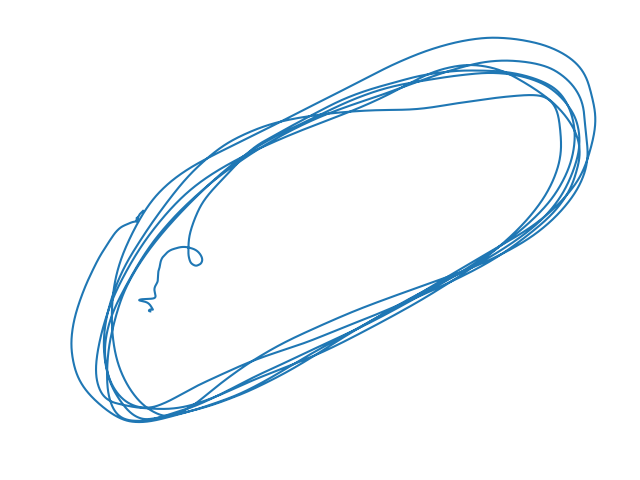
\includegraphics[width=0.35\textwidth]{indoor_forward_3.png}
    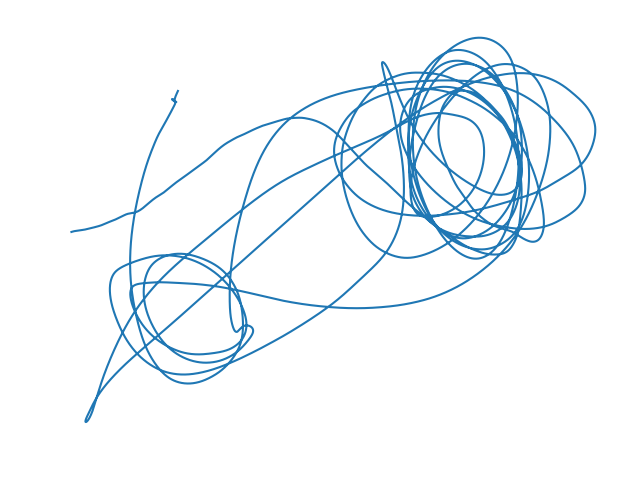
\includegraphics[width=0.35\textwidth]{indoor_forward_7.png}  \\
    \caption{Example flight trajectories from the UZH FPV Dataset \cite{Delmerico19icra}}
    \label{DatasetExamples}
\end{figure}

\section{Approach}
\paragraph{The Transformer}$ $
\\Transformers have shown great success with sequential tasks in NLP and other domains \cite{attentionisallyouneed}. They also offer parallelization making them faster than recurrent approaches like LSTMs. This makes them a good fit for my task given the sequential nature of trajectories and the need for speed of inference in a drone race. The purely transformer-based approach introduced by \cite{giuliari2020transformer} for pedistrian trajectory prediction achieved state of the art results for that task. Therefore, I'm using their approach as the baseline and backbone of my GAN-based approach.

\paragraph{The Adversarial Loss}$ $
\\The baseline transformer uses MSE loss given the spacial nature of the data. However, adversarial loss allows for our desired diversity in the output. Figure \ref{gen_disc_figure} shows my proposed architecture which uses the transformer as a generator that takes in the positional history $x_{i-n}...x_{i-1}, x_{i}$, concatenated with random seeds, and the temporal embedding proposed in \cite{giuliari2020transformer} as input. While the decoder generates a trajectory $y_0, y_1, ... y_m$. 
\\ The discriminator is an encoder that takes the concatenated sequence making the candidate trajectory and gives it a fakeness score as insipred by \cite{fakereviewsgan}. These two components make a complete GAN that can be trained with BCE loss to generate diverse predicted trajectories.

\begin{figure}
    \centering
    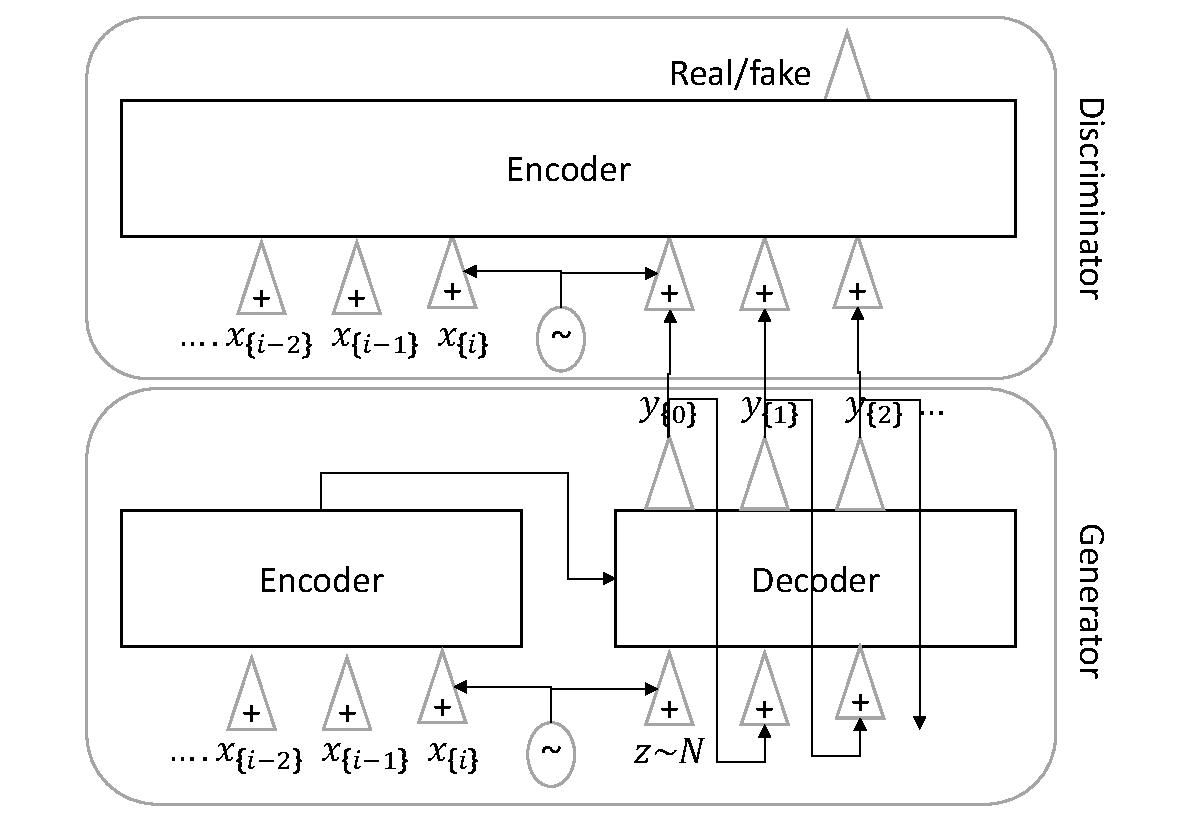
\includegraphics[width=0.45\textwidth]{gen-disc-figure.pdf}
    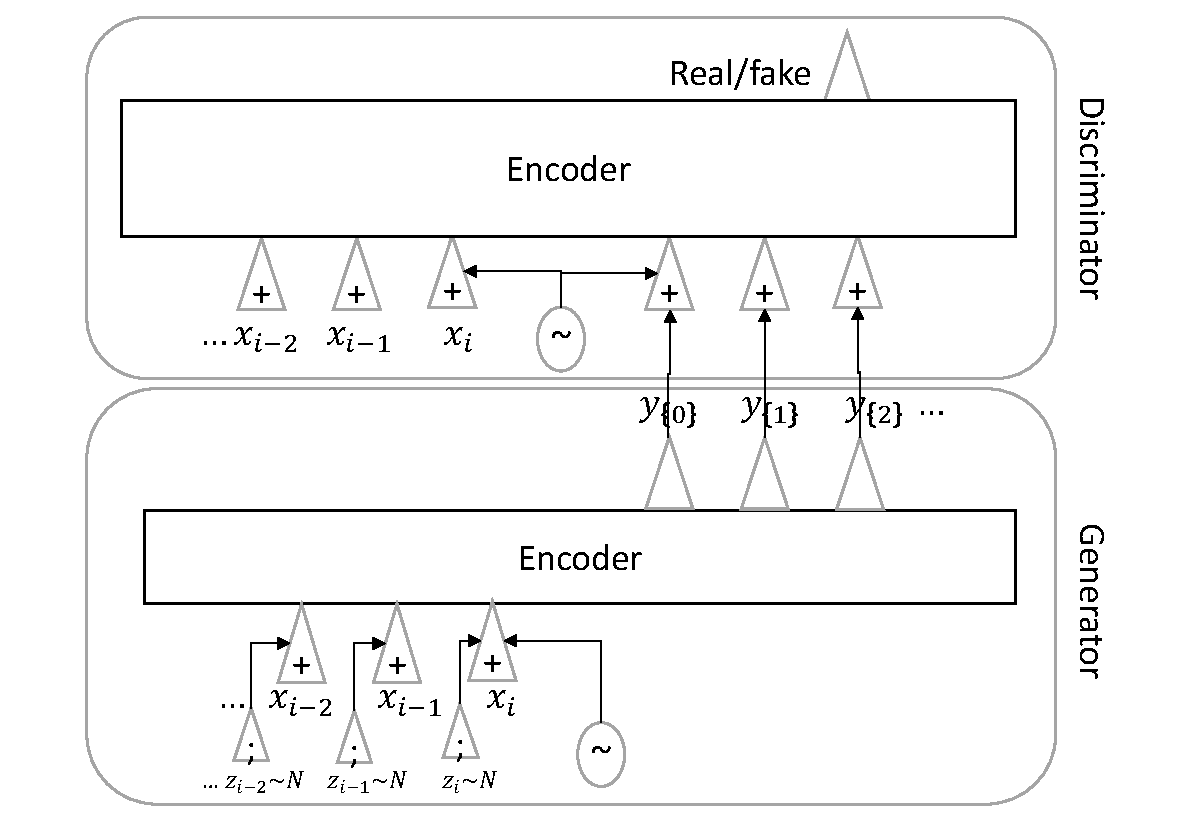
\includegraphics[width=0.45\textwidth]{gen-disc-parallel-figure.pdf}\\
    \caption{The proposed GAN architecture.  The circle represents the temporal embedding for each timestep as proposed in \cite{giuliari2020transformer}.  Left is the original proposal, Right is the new parallelized one.}
    \label{gen_disc_figure}
\end{figure}

\paragraph{Evaluation}$ $
\\I would like the predicted trajectory to be similar to the ground truth. The literature \cite{giuliari2020transformer} uses the Mean Average Displacement MAD and the Final Average Displacement FAD. The latter of which averages the distance of the final state of the predicted trajectory from the final state of the ground truth, while the former does the same averaging over all the points of the trajectories. 
\\Since we desire diversity in the GAN output, it is not fair to penalize it for the trajectories that don't match the ground truth. Therefore, I propose to consider only the minimum MAD and FAD over a batch of generations with diverse random vectors for the same history sequence. I could also experiement with the truncation trick to produce predictions with high fidelity and treat them the same way as the single-prediction baseline.  
\\To measure the diversity of the GAN outputs, I propose to use a clustering algorithm (e.g. k-means) over its output on a batch of random vectors for the same history sequence and find the distance between these clusters.  This metric is very loose because I'm not comparing the model diversity to the baseline, but it's a good indicator that there's at least some diversity in the generations. 

\section{Experiments and Results}
\paragraph{The Baseline}$ $
\\I trained the simple transformer baseline using the same implementation linked in \cite{giuliari2020transformer} with the training dataset for 130 epochs in 30 minutes on a Tesla K80. The batch size was 64 and the number of validation frames was 64 per flight (as described in the dataset section of this report).  I also requested that the model be evaluated on the test set on every epoch for more insight given the small size of the validation set and ended up with both evaluations yielding almost identical curves with better results on the test set.  Figure \ref{baseline_train_loss} shows the results and a few visualized samples. 

\begin{figure}
    \centering
    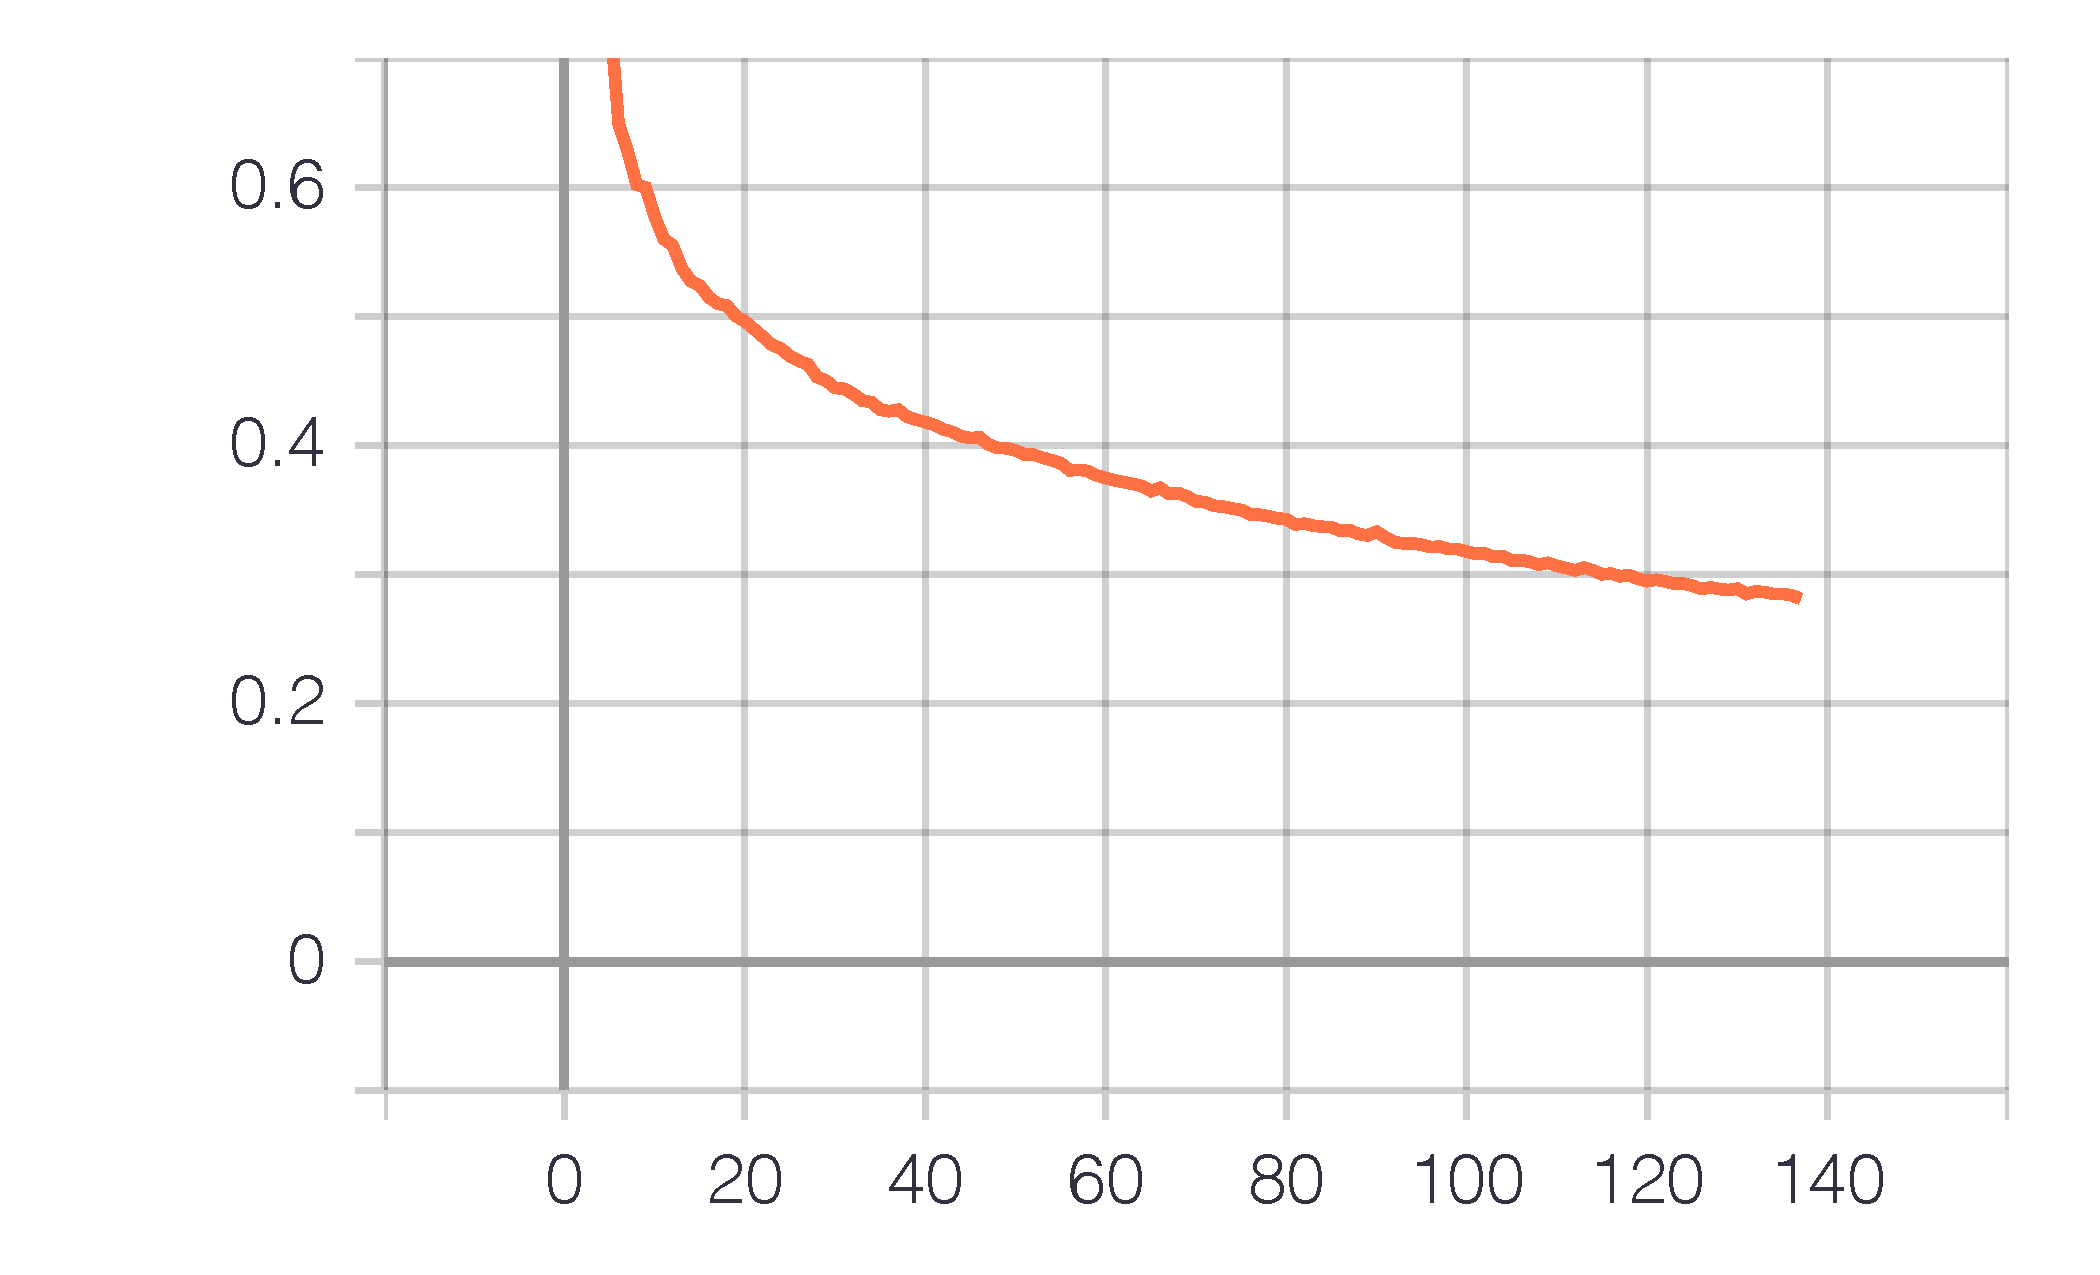
\includegraphics[width=0.45\textwidth]{loss_train_baseline_long.pdf}
     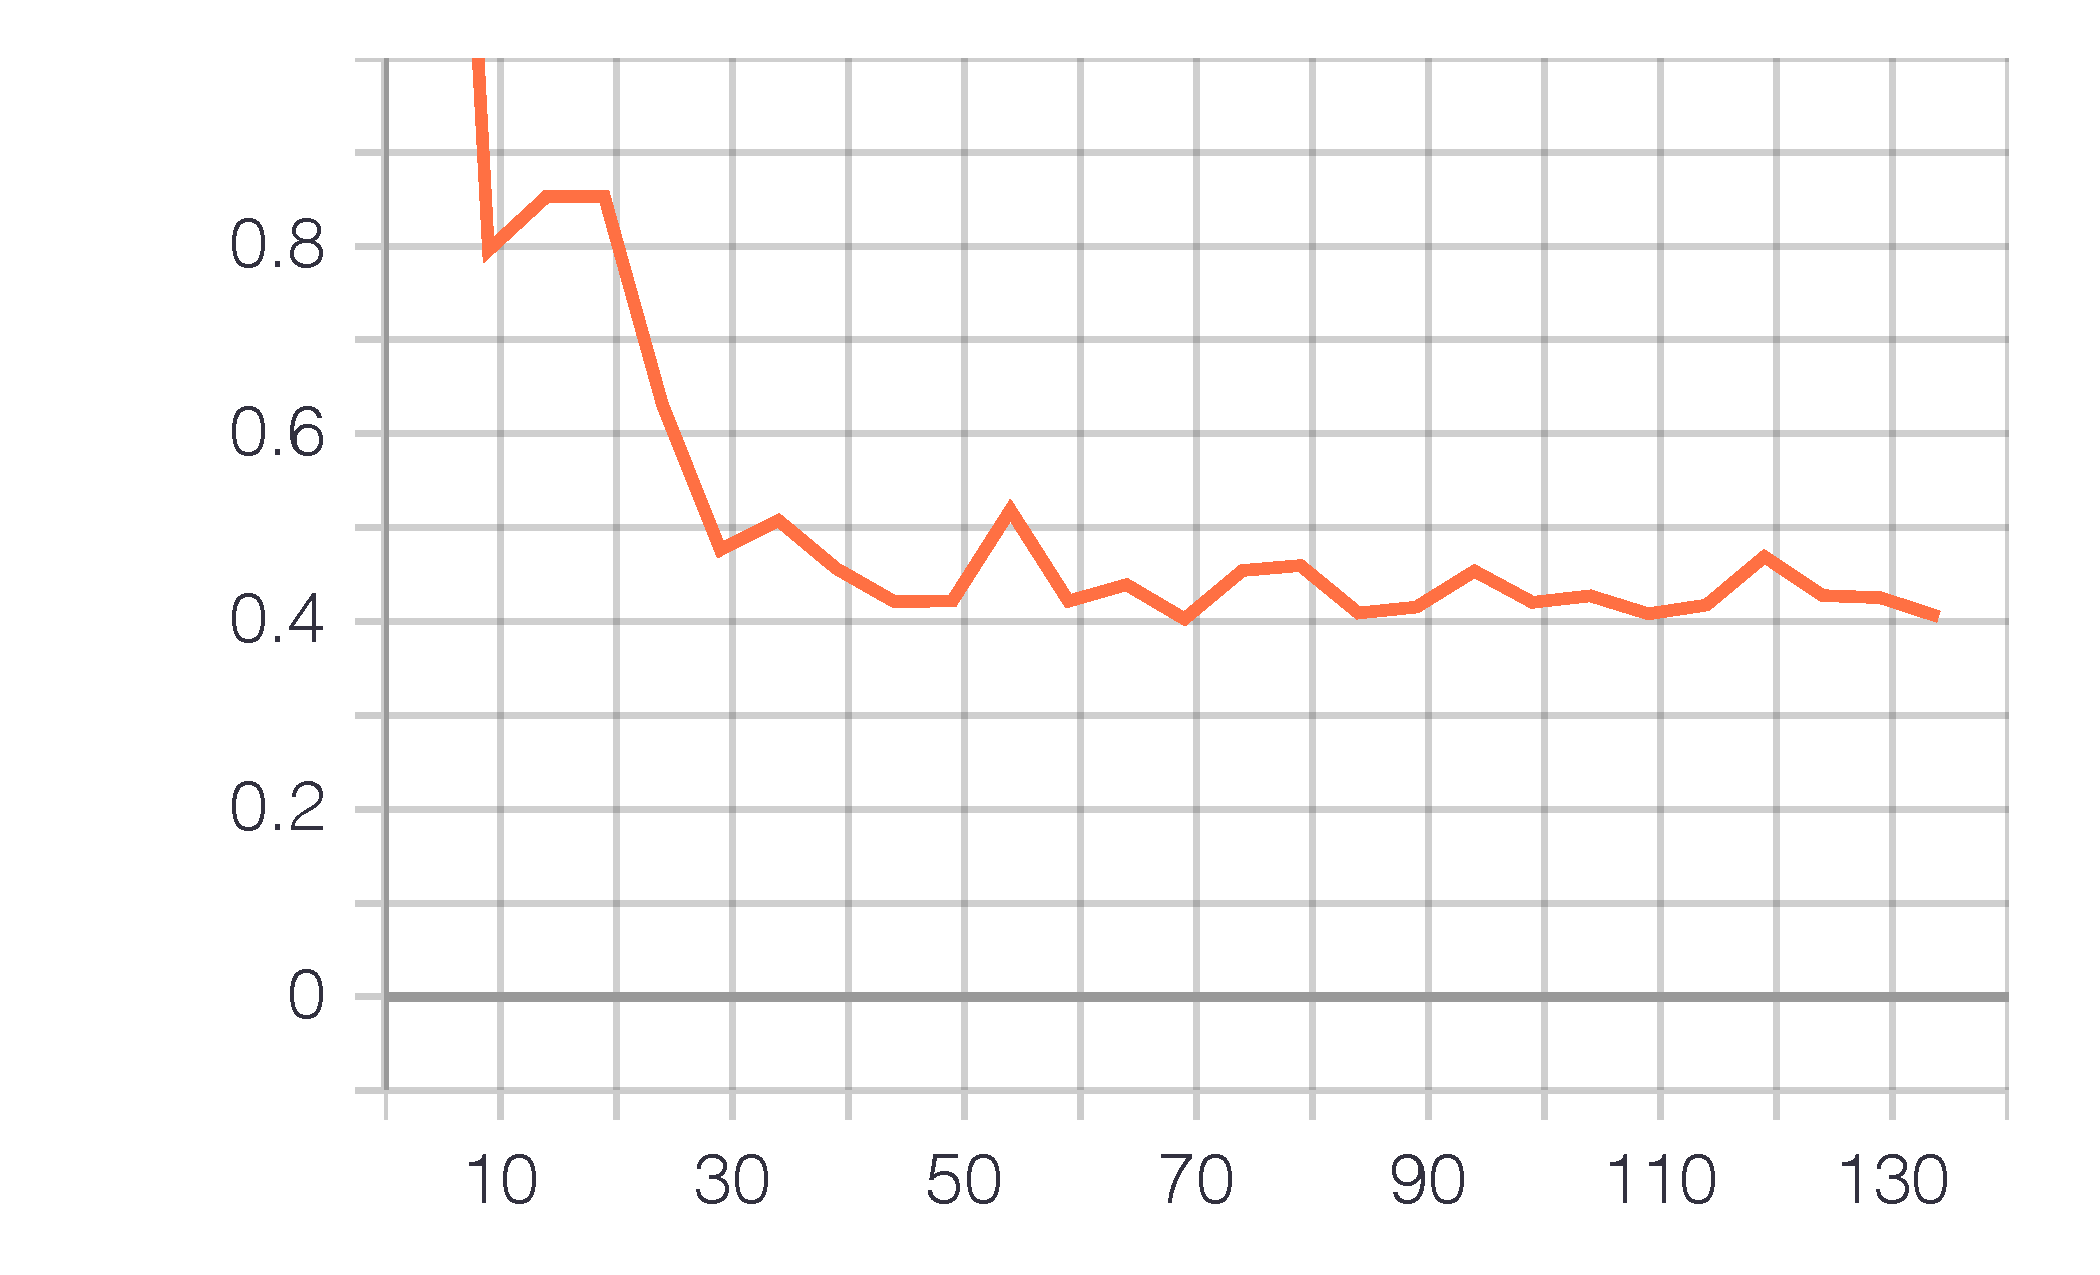
\includegraphics[width=0.45\textwidth]{test_mad_train_baseline_long}\\
    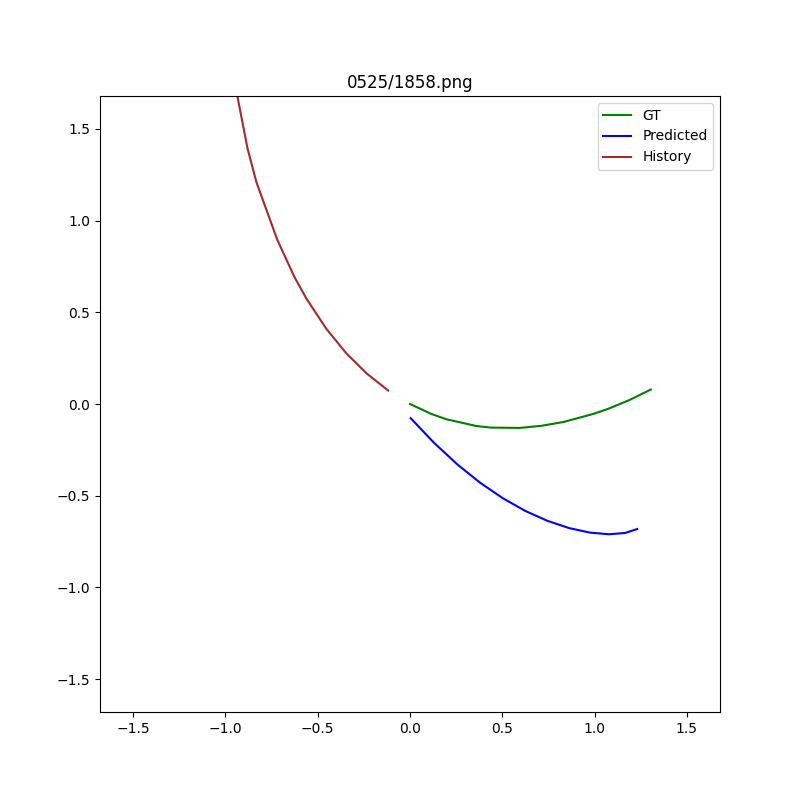
\includegraphics[width=0.3\textwidth]{baseline0}
    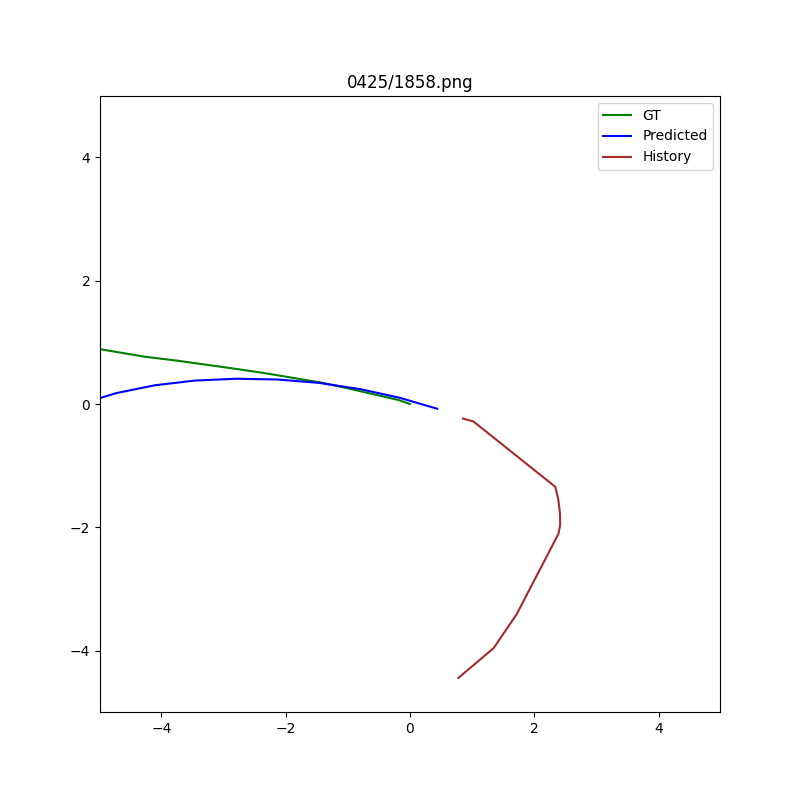
\includegraphics[width=0.3\textwidth]{baseline1}
    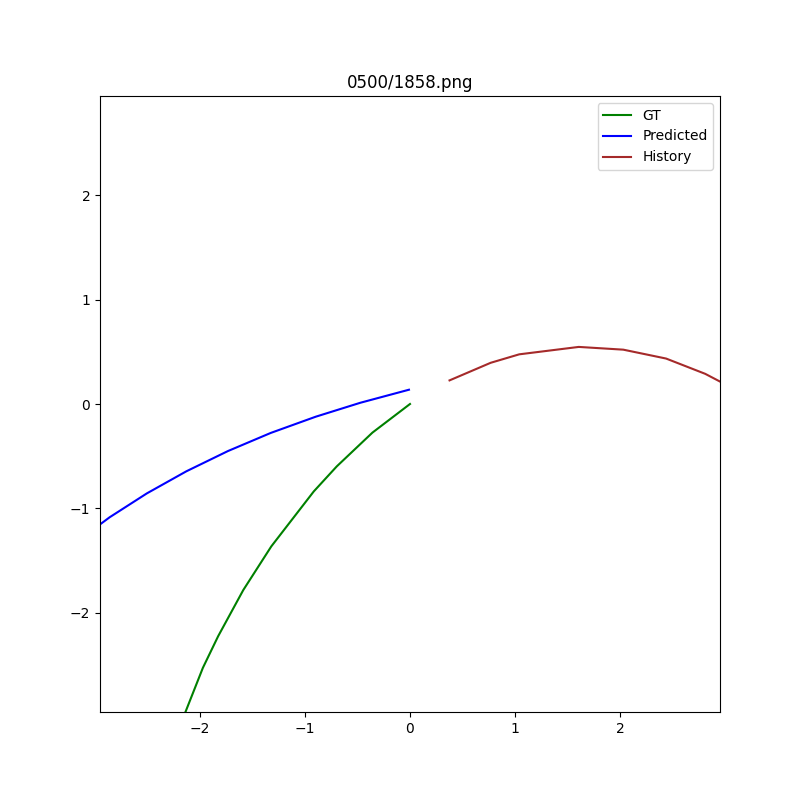
\includegraphics[width=0.3\textwidth]{baseline2}\\
    \caption{The x axis is the epoch. The left chart is the average loss per epoch. The right chart is the MAD on the test set at each epoch. On the second row are example outputs: brown is the input, green is the gound truth, and blue is the prediction.}
    \label{baseline_train_loss}
\end{figure}

\paragraph{GAN-Based}$ $
\\I implemented GAN-based model I proposed shown in Figure \ref{gen_disc_figure} (left) and trained it on the same dataset using Wasserstein Loss \cite{wloss} with multiple values of gradient penalty and critic repetitions. The training curves are shown in Figure \ref{sequential_training_loss}. Training took longer than for the baseline because of the sequential unfolding of the generator's decoder (coming from the assumption that we don't have ground truth for the generation task).  This sequential nature also led to vanishing gradient for the generator where it didn't learn past the random weights it was initialized on, leading to mode collapse in the generations. Some examples are shown in Figure \ref{sample_mode_collapse}.
\begin{figure}
    \centering
    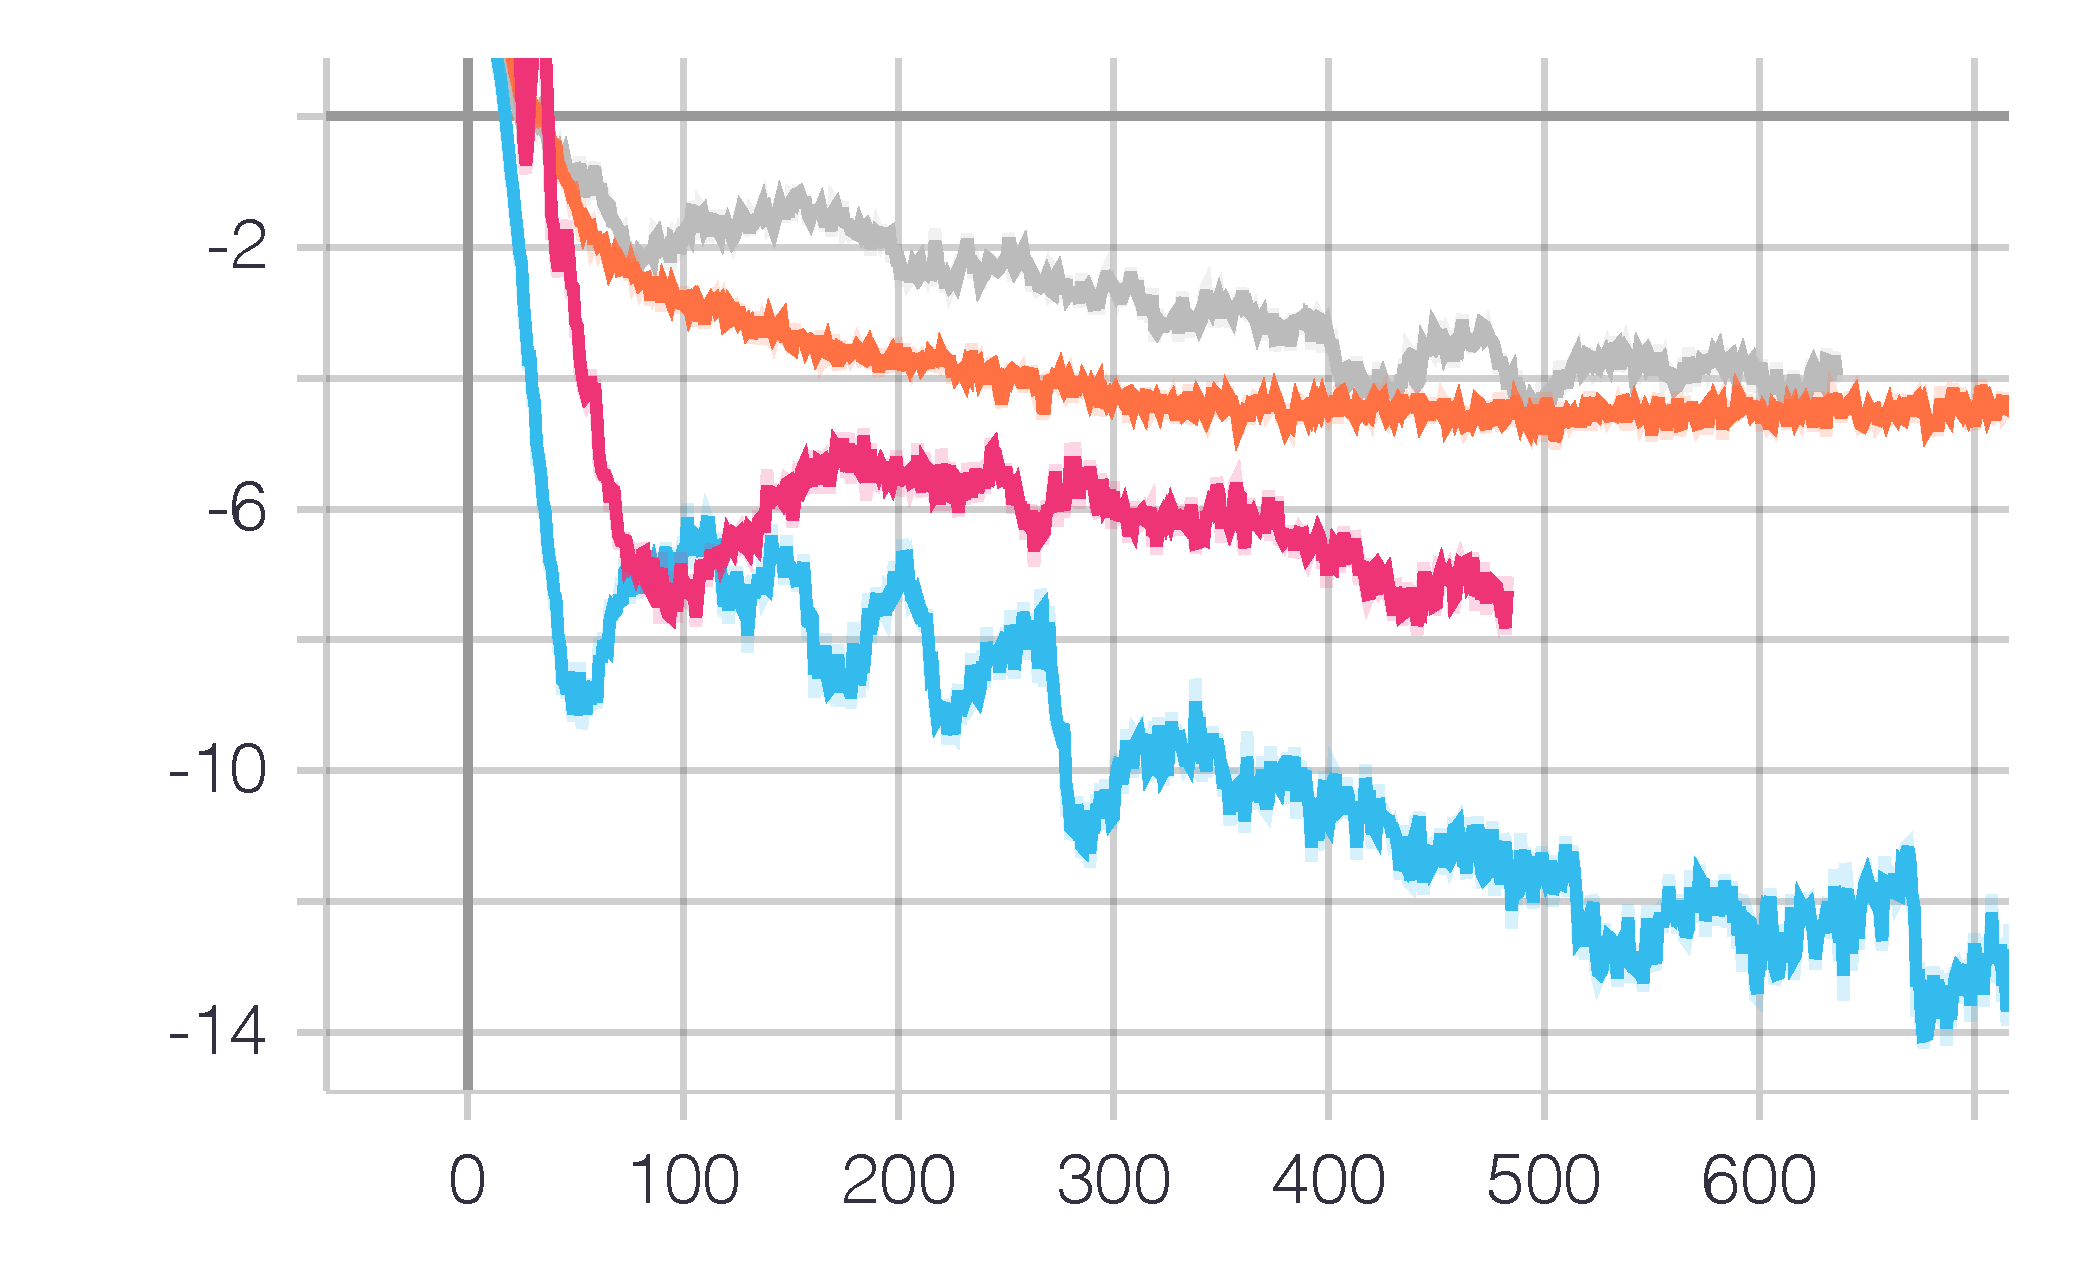
\includegraphics[width=0.45\textwidth]{Loss_train_crit_collapse}
     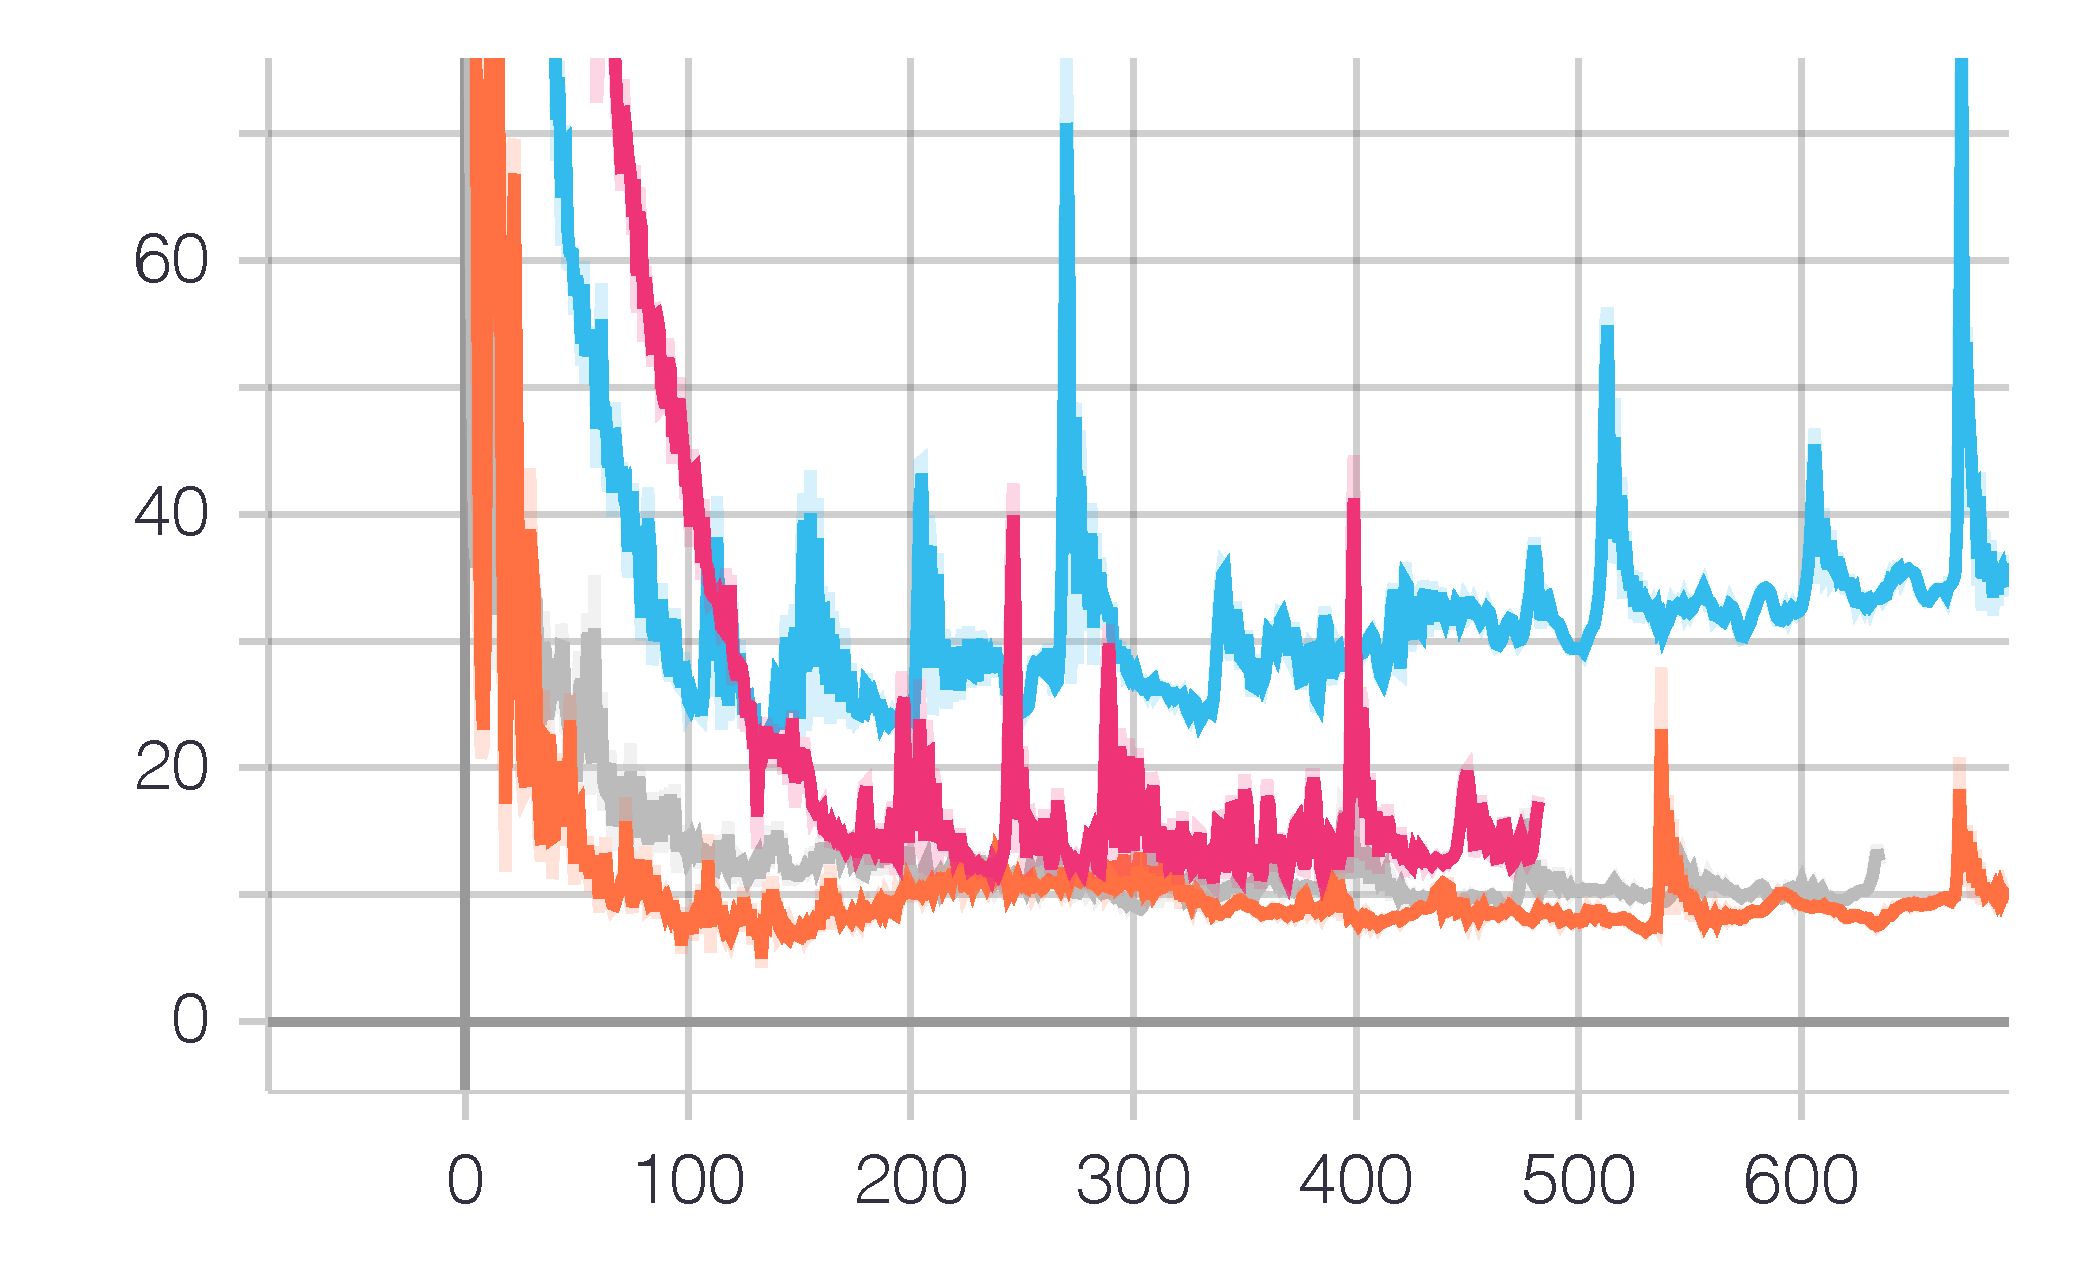
\includegraphics[width=0.45\textwidth]{Loss_train_gen_collapse}\\
    \caption{W-Loss curves for Critic on the left and Generator on the right with batch on the horizontal axis. \textbf{Cyan} is \textbf{G}radient \textbf{P}enality of 10 and \textbf{W}indow of 8; \textbf{Magenta} is \textbf{GP} of 100 and \textbf{W} of 8; \textbf{Grey} is \textbf{GP} of 10 and \textbf{W} of 2; \textbf{Orange} is \textbf{GP} of 10 and \textbf{W} of 1 }
    \label{sequential_training_loss}
\end{figure}

\begin{figure}
    \centering
    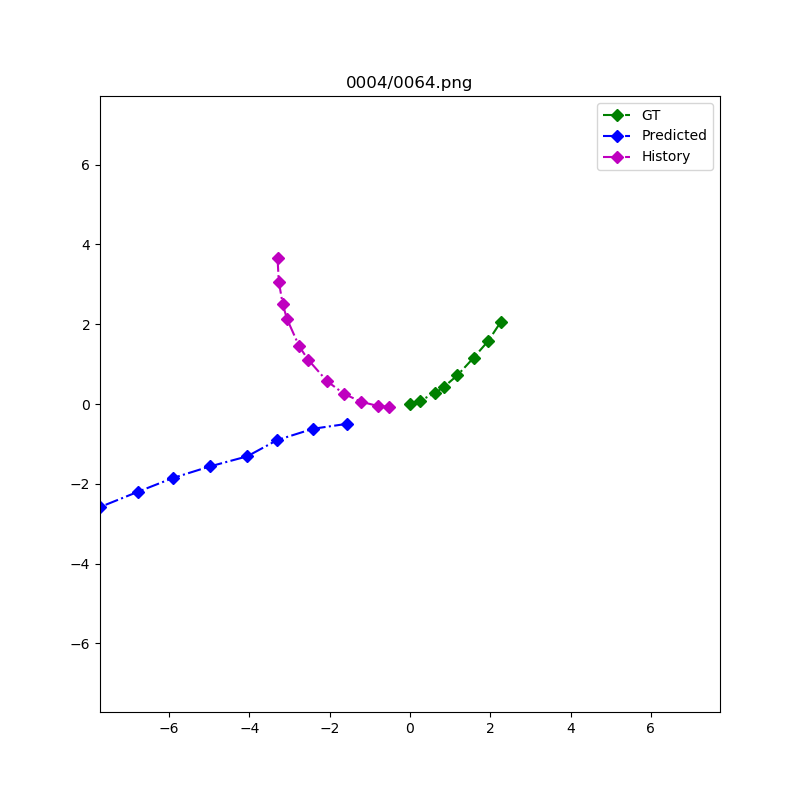
\includegraphics[width=0.3\textwidth]{mode_collapse0}
    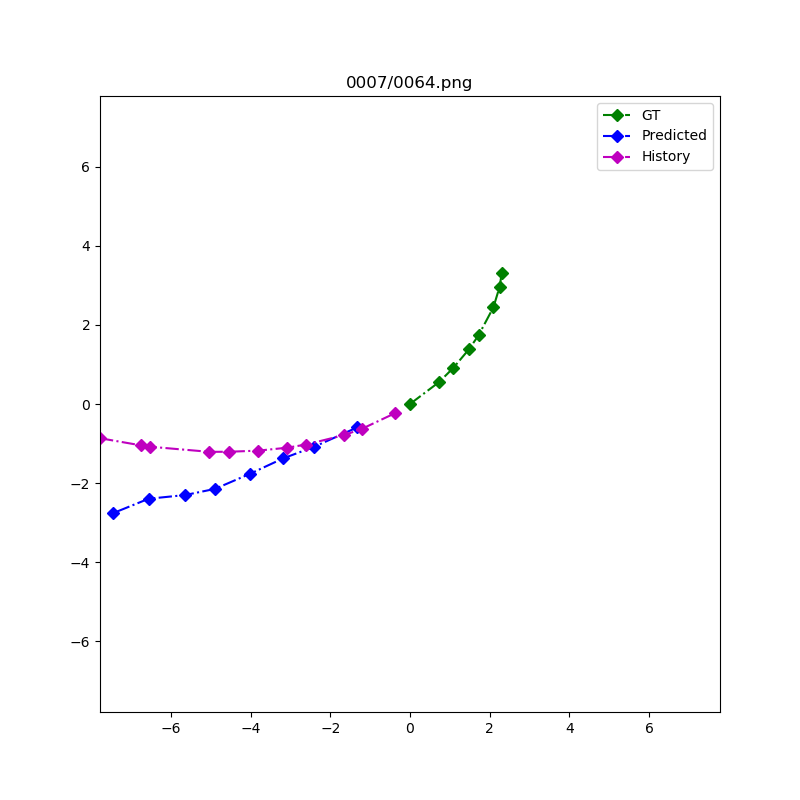
\includegraphics[width=0.3\textwidth]{mode_collapse1}
    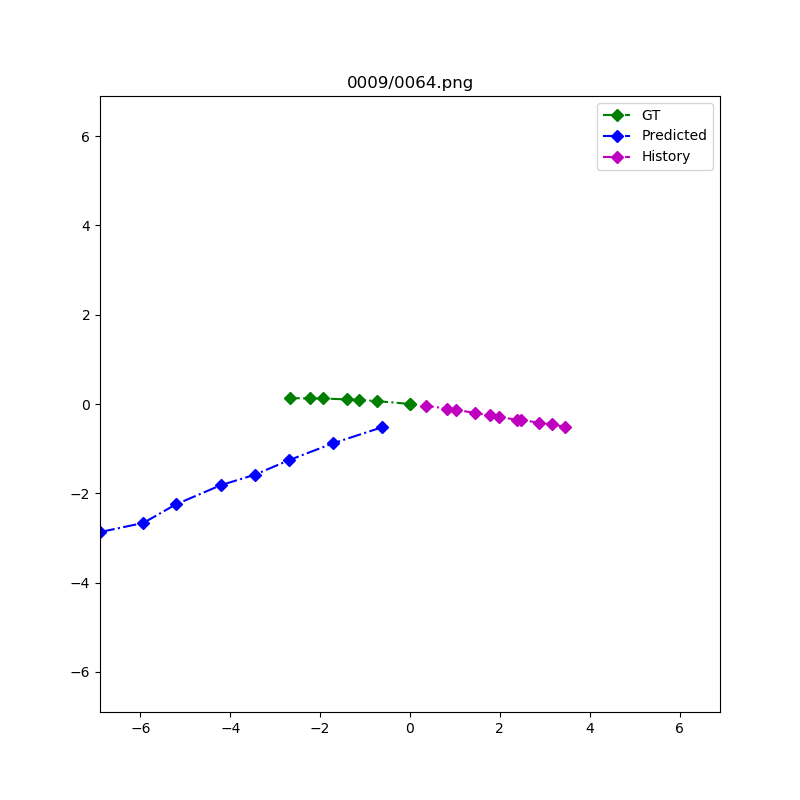
\includegraphics[width=0.3\textwidth]{mode_collapse2}\\
    \caption{A few samples generated by the generator during training. Magenta is the condition input sequence, Green is the real trajectory, and Blue is the generated trajectory. Notice how similar all the blue trajectories are for various conditions.}
    \label{sample_mode_collapse}
\end{figure}

\paragraph{Analysis}$ $
Looking at the loss curves in Figure \ref{sequential_training_loss}, we find two things:
\begin{itemize}
\item Higher Gradient Penality allows the generator to learn more by slowing down the critic as the Cyan and Magenta curves are flipped for the Critic and Generator.
\item Smaller trajectory window (unfolds of the generator) lead to better training and smaller loss for the generator.  This is probably due to the vanishing gradient happening during the unfolding process for long sequences.
\end{itemize}

\paragraph{Improved GAN-Based}$ $
\\
This leads to the conclusion that I should get rid of the sequential unfolding in the generator and to incorporate the injected noise better into the generator. Therefore I propose another approach shown in figure \ref{gen_disc_figure} (Right) where there's no sequential unfolding. Instead, the decoder is abandoned for a simple Encoder-only transformer (similar to BERT) where the noise is concatenated to the input states. \\
I also add an additional reconstruction loss term for the generator which is a scaled MSE loss. It's important to keep this scaled minimally so it doesn't reduce the variaty of the generations even though it boosts its fidelity. 
I ran training for the new method for 3 hours with the losses shown in figure \ref{encoder_only_training}. That is 78 epochs.  The reconstruction loss was weighted by a factor of 2 which I chose after experimenting with $0.1$ and $1$.  Notice that the model doesn't stop improving at that point but I had to stop the training because of the time constraint.  Some examples are shown in Figure \ref{only_encoder_samples}.

\paragraph{Analysis}$ $
\\Looking at the loss curves in Figure \ref{only_encoder_samples}, we find two things:
\begin{itemize}
\item The new architecture solved the mode collapse problem and the predicted trajectories are not identical to each other anymore.
\item The predicted trajectories have a problem with scale and the generations are too small spacially even with the reconstruction loss. There are multiple solutions to try for this. One is to increase the reconstruction loss weight. Another one is to normalize the input of the generator and rescale it to the original for the output. This is similar to instance normalization but with the additional step of scaling up/down to the original again at the output layer. 
\end{itemize}





\begin{figure}
    \centering
    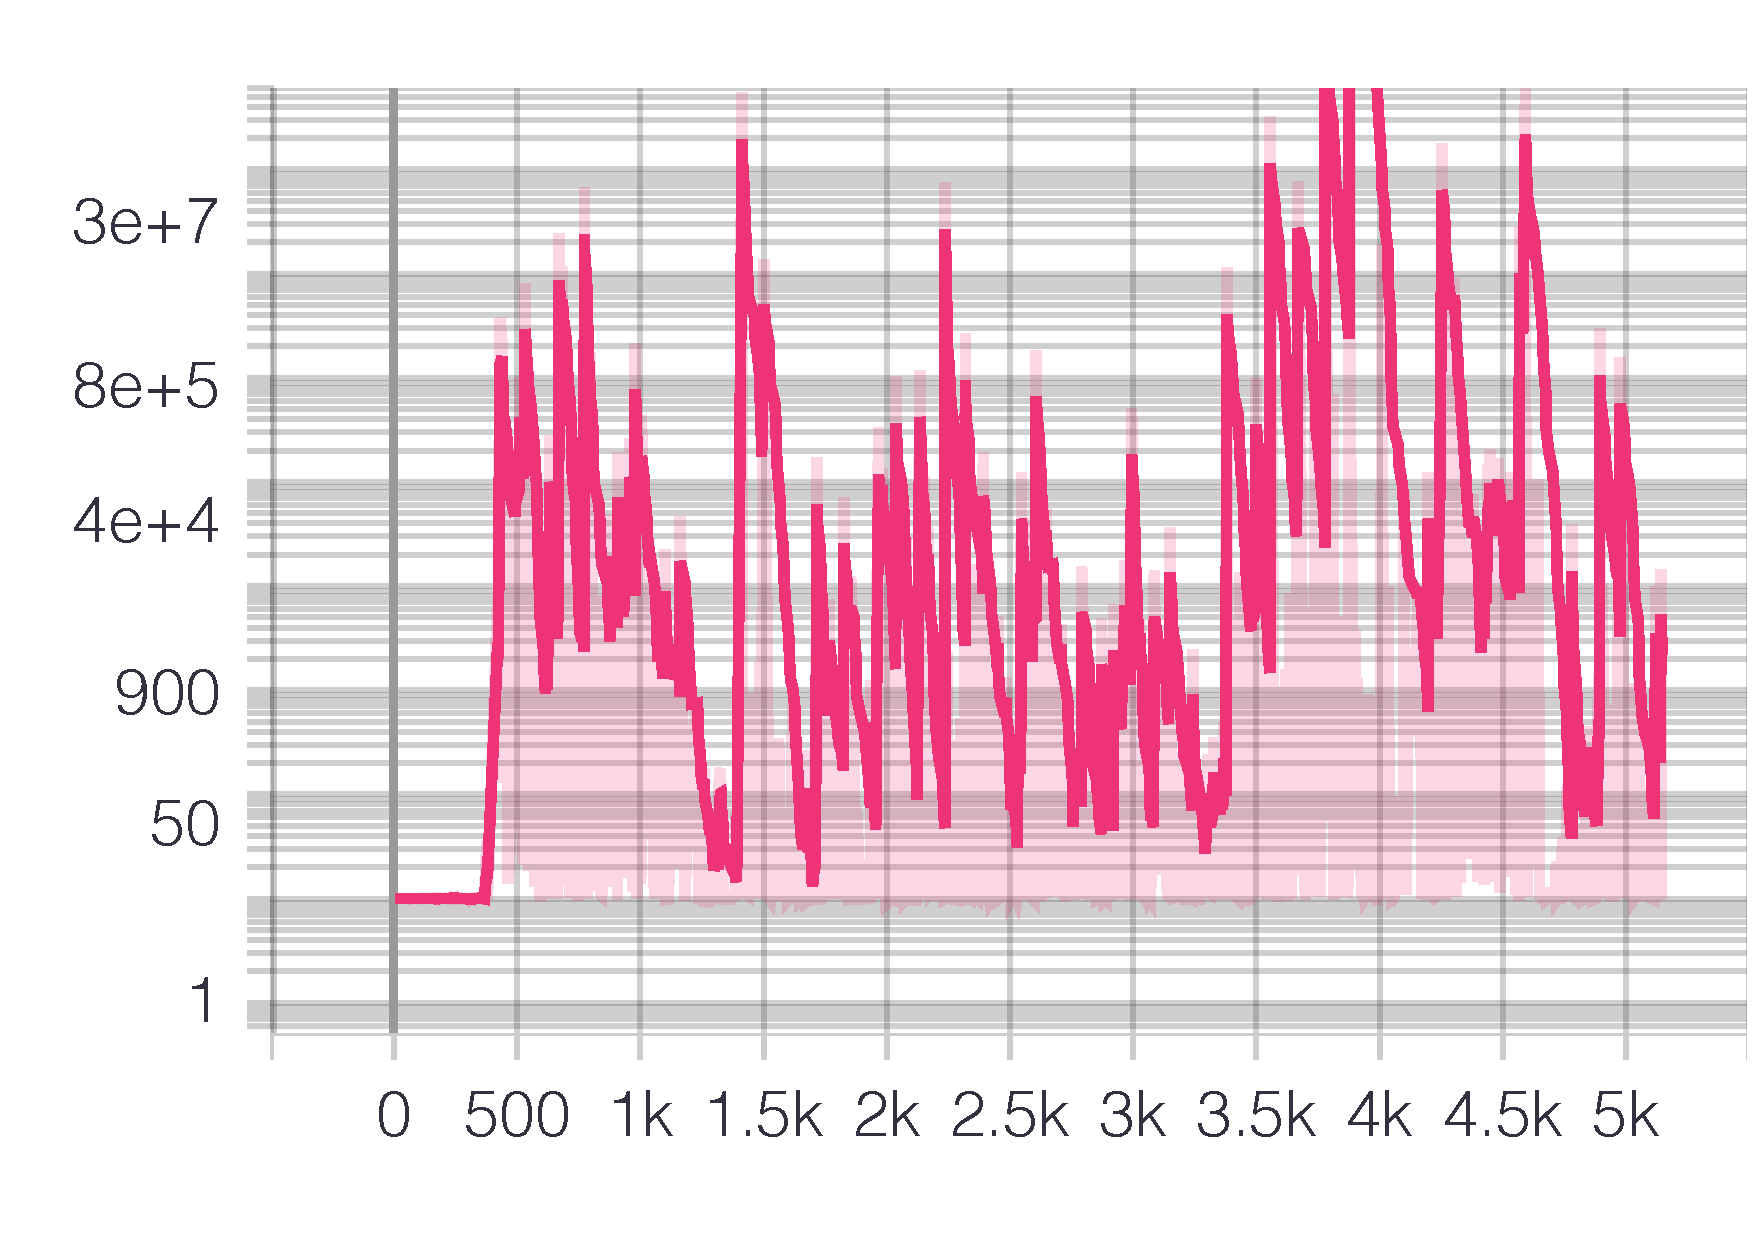
\includegraphics[width=0.45\textwidth]{Loss_train_crit_enc}
     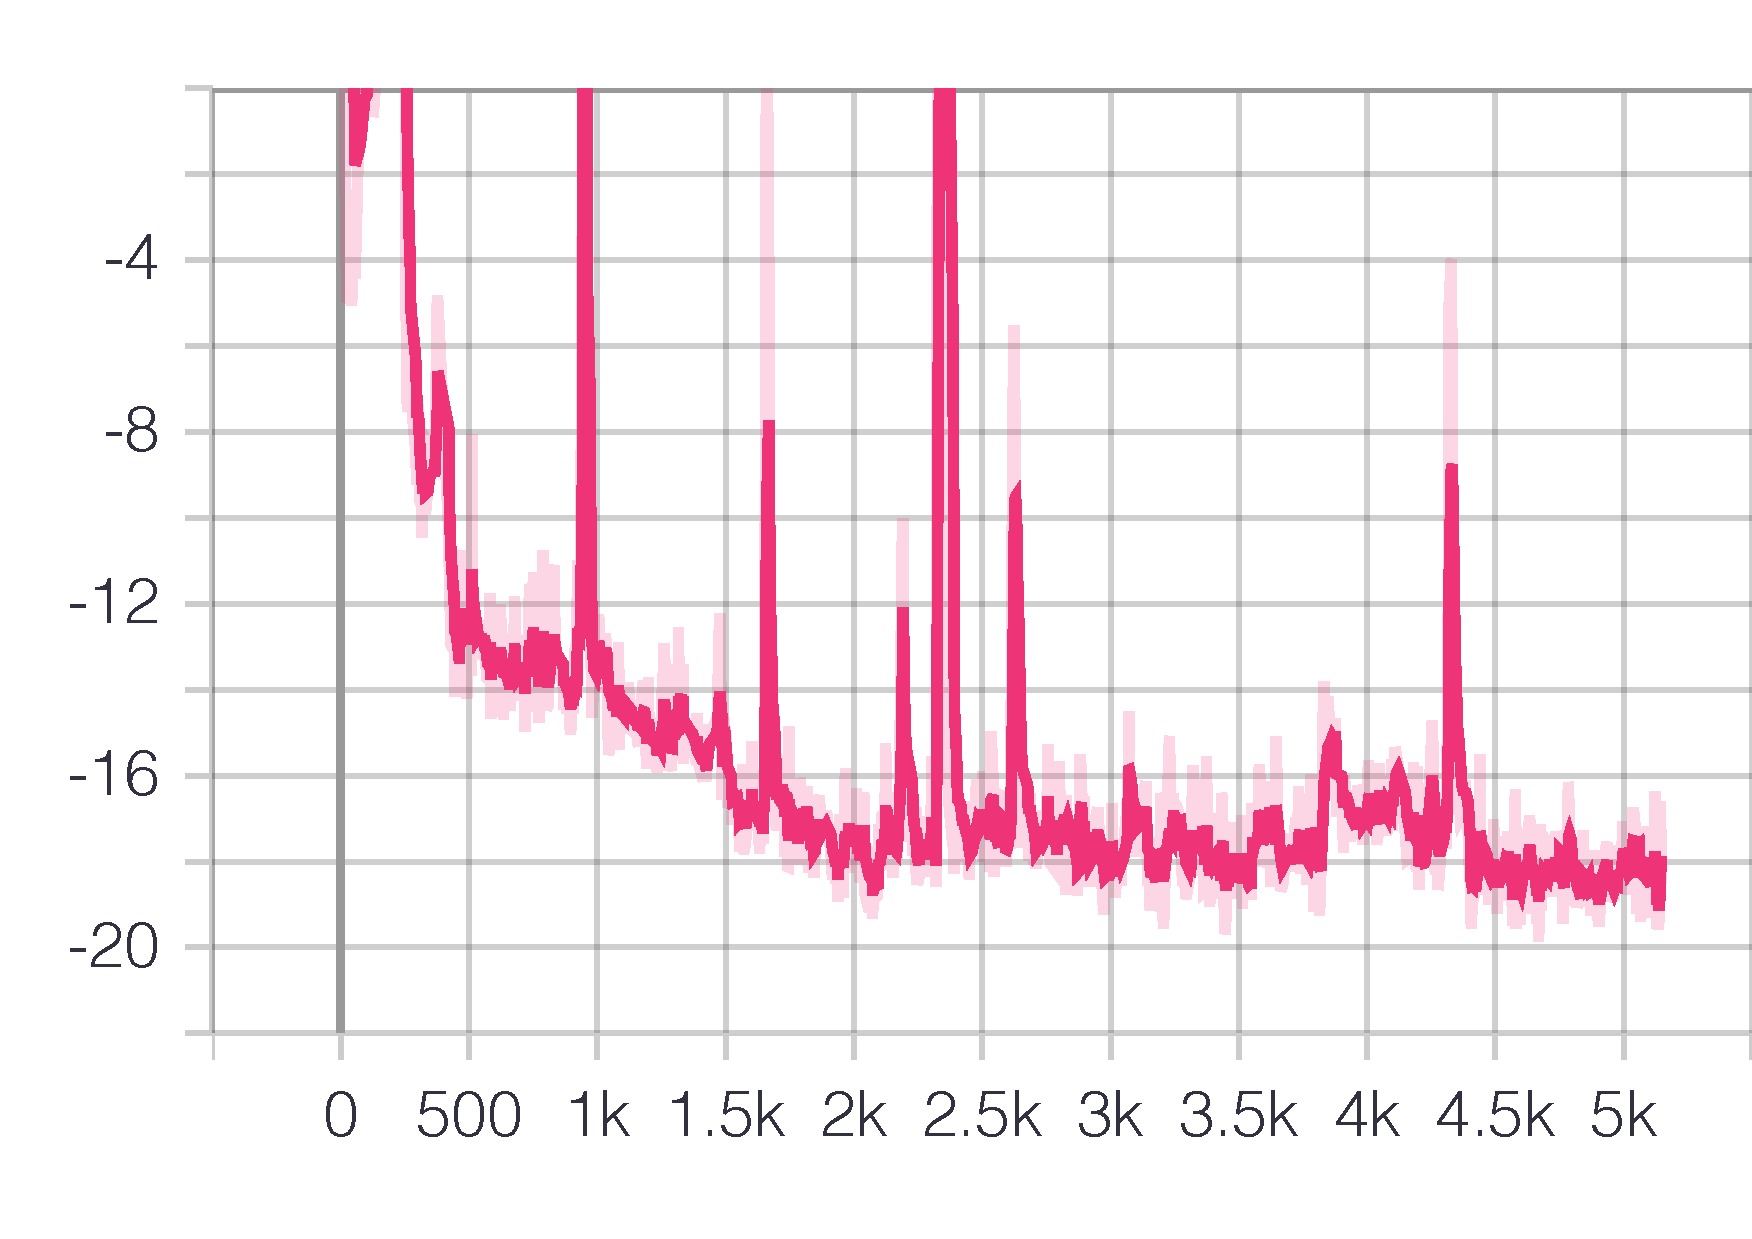
\includegraphics[width=0.45\textwidth]{Loss_train_gen_enc}\\
    \caption{W-Loss curves for Critic on the left and Generator on the right with batch on the horizontal axis.  Notice that learning still hasn't plateaued by the end.}
    \label{encoder_only_training}
\end{figure}

\begin{figure}
    \centering
        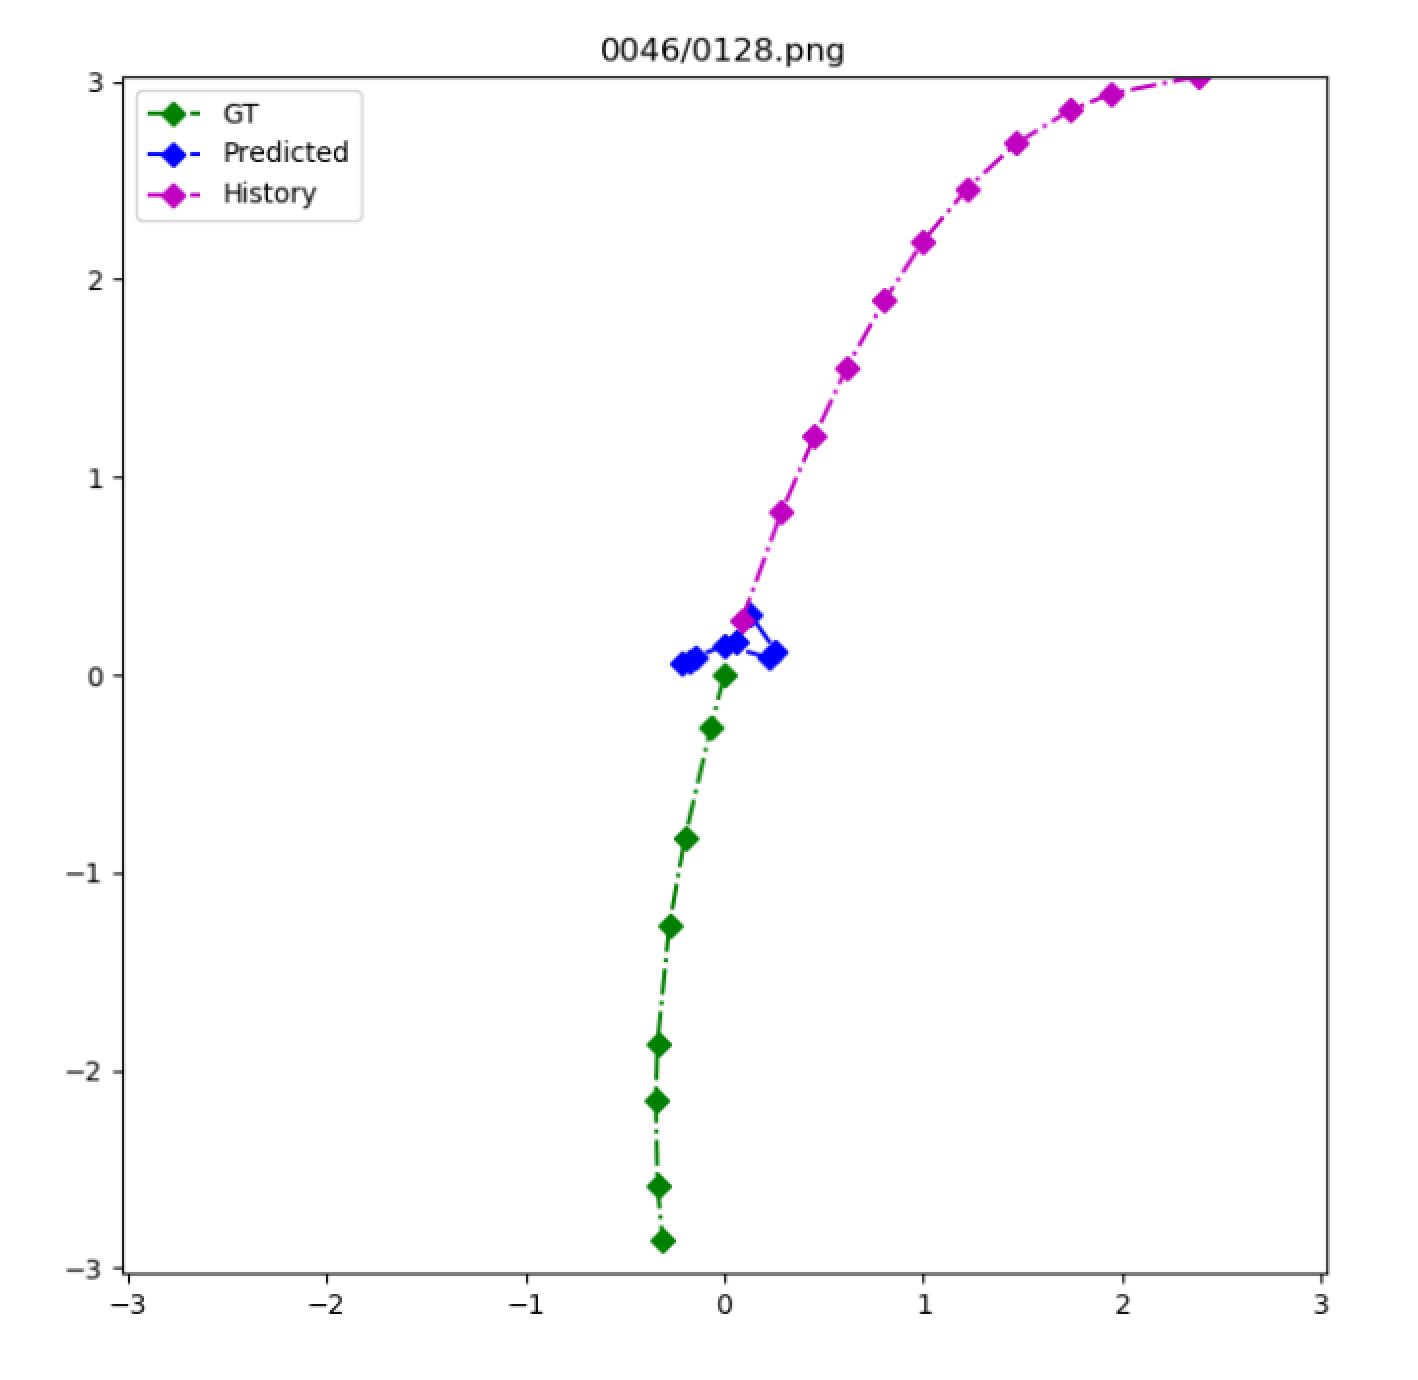
\includegraphics[width=0.3\textwidth]{encoder_only_1}
    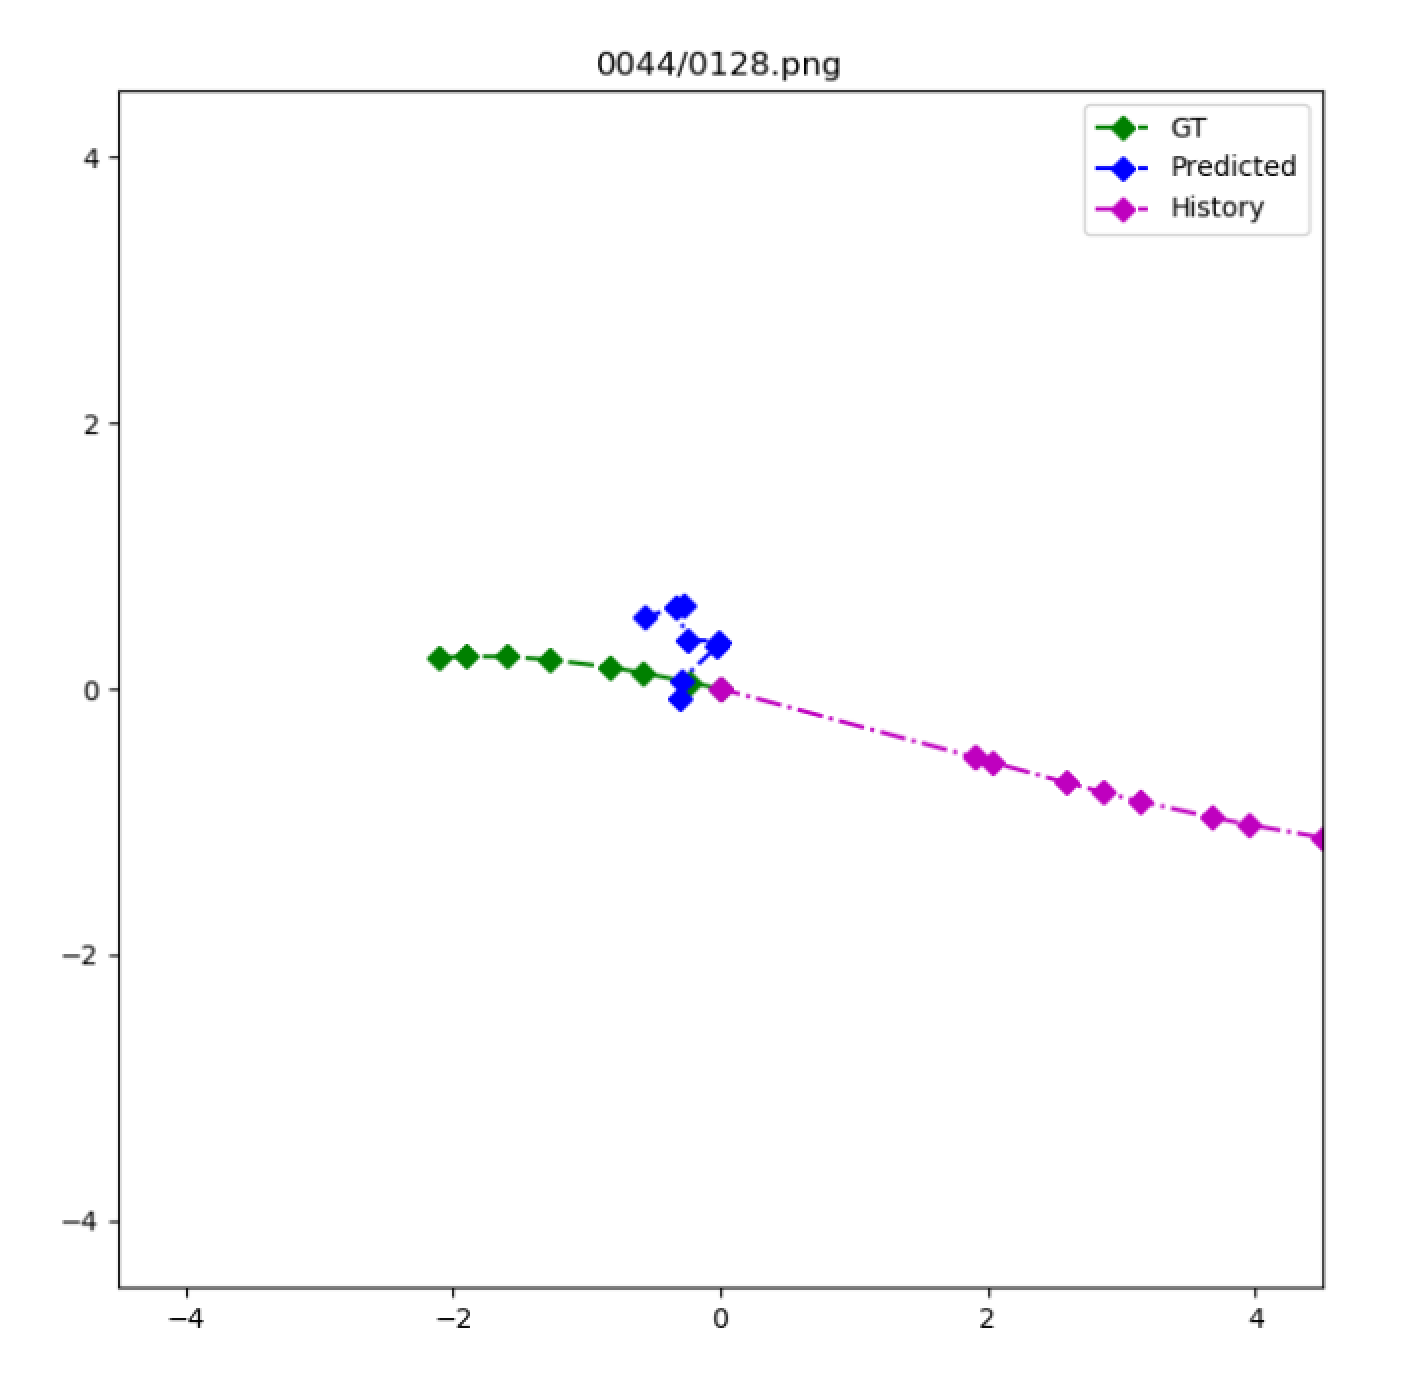
\includegraphics[width=0.3\textwidth]{encoder_only_2}\\
    \caption{A few samples generated by the generator during training. Magenta is the condition input sequence, Green is the real trajectory, and Blue is the generated trajectory. Notice that blue is clustered around the end of the trajectory.}
    \label{only_encoder_samples}
\end{figure}

%\section{Moving Forward}
%After evaluating the original proposed method, I will implement the new method and evaluate it in a similar way. I will measure the fidelity and variaty of the generations using the metrics I proposed earlier. After that, I would like to try the following risky experiments:

\paragraph{Risky Experiments}$ $
\begin{itemize}
\item Request a longer prediction horizons and use that to measure how over-fit the model could be. Because the past trajectory of an object doesn't necessarily contain enough information about the future, if the model gets good results, it means that it's leaking information from the training set.
\item Set all the input states as random values and see how well the model performs on that. Good accuracy on that implies that the model doesn't depend heavily on the input but instead gives a general prediction regarless of the condition. 
\item Preprocess the coordinates of a drone during flight as seen from another drone during a concurrent flight (this doesn't exist in the dataset but we can assume that two flight recordings were happening at the same time and with the same coordinate reference/calibration). This will show us if the model actually generalizes to do the task when it's on a moving drone in a race rather than on a stationery sensor.
\end{itemize}



\bibliographystyle{unsrt}
\bibliography{references}

\end{document}
